\begin{flushright}

\end{flushright}\section{Performance Evaluation}
\label{sec_perf}
 

\subsection{Simulator Overview}
To evaluate the performance and power consumption of the proposed
architecture, we simulate the multi-core heterogeneous architecture
by extending Multi2Sim - a superscalar, multithreaded and multicore
simulator - with a reconfigurable accelerator unit. 
 The specification of our simulated architecture is shown in Table
\ref{tbl_parameters}. The processor core technology and operating
frequency is modeled based on the Atom 330 processor, and we set the
number of cores as eight in the baseline configuration. Later we vary the
number of cores to explore the area allocation to accelerators and cores. 
The ICAP interface runs at 100 MHz although over-clocking ICAP is
possible in practice\cite{Hansen:2011dt}.

\begin{table}
\scriptsize
\begin{center}
  \begin{tabular} { | l | l | }
    \hline
    \textbf{Item} & \textbf{Parameter} \\
    \hline
    \hline
	Core & 8 \\
	\hline
	Core Spec & 45nm @ 1.6 GHz \\
	\hline
	Accelerator Spec& 45nm @ 200 MHz \\
	\hline
	ICAP & 32 bit bus width @ 100 MHz \\
	\hline
	L1 Instr/Data Cache Size (KB) & 32 \\
	\hline
    L1 Instr/Data \$ Associativity & 4\\
    \hline
    L1 Instr/Data \$ Block Size (Bits) & 64\\
    \hline
    L1 Instr/Data \$ Number of Sets & 128\\
    \hline
    L1 Instr/Data \$ Latency (Cycles) & 3 \\
   	\hline
   	L2 Cache Size (MB) & 4 (shared) \\
   	\hline
    L2 Associativity & 8\\
    \hline
    L2 Block Size (Bits) & 512\\
    \hline
    L2 Number of Sets & 1024 \\
    \hline
    L2 Latency (Cycles) & 20\\
    \hline
    CPU Cache Coherence & MOESI\\
    \hline 
    Accelerator Data Buffer Coherence & MOESI\\
    \hline
    Memory Size (GB) & 8 \\
    \hline
    Memory Latency (Cycles) & 200 \\
    \hline
    Memory Data Block Size (Bytes) & 512\\
    \hline
    Memory Page Size (Bytes) & 8192\\
    \hline
    Memory Replacement Policy & Pseudo LRU\\
    \hline
    Network Topology & 2-D Mesh\\
    \hline
    Network Bandwidth (MB/s) & 1024\\
    \hline
  \end{tabular}
\caption{Hardware Specification.}
\label{tbl_parameters}
\end{center}
\end{table}


To model the profiling and scheduling overheads in the simulations,
we evaluate the overhead of the profiler within the wrapper function and the
three scheduling methods - na\"{\i}ve, bandwidth first or speedup first. For
the worse case, the profiler and wrapper function overheads take up
to 0.017 \% per profiling window time and the worse case happens only
when the reconfiguration controller accepts the current acceleration
request within the profiling window. The two knapsack combination
scheduling algorithms introduce more overhead than na\"{\i}ve scheduling. However, further evaluation shows that the overhead of both bandwidth
first and speedup first algorithms introduce an neglectable overhead of 0.130 \% per profiling window. 

\subsection{Benchmarks}
We use all the eight acceleration functions from the
open-source accelerator store \cite{accstore} to build a synthetic
workload that simulates dynamic workloads in cloud and mobile
environments (we defer using real-world cloud applications to our
future work).  These applications cover a wide range of areas
including encryption/decryption ({\em 3DES} \cite{openssl}), numerical
calculation ({\em Jacobi} \cite{jacobi-wiki}), vision and navigation
({\em SLAM-C and SLAM-J} \cite{openslam}), feature detection (SURF and
IDSI \cite{opencv}), image processing ({\em Segmentation}
\cite{segmentation-wiki}) and bioinformatics ({\em Smith-Waterman}
\cite{smithwaterman-wiki}). Besides, these software applications have
corresponding accelerator implementation which provide
performance/area details. Minor modifications are done to generate the
final benchmark mixture, including preparing the input data set for
each function and creating multiple threads.

To emulate the dynamics of workload arrival, we model the inter-arrival time of
requests to an accelerated function as a Poisson process. The average
inter-arrival time is set as 500,000,000 (312.5 ms
in real time if system is running at 1.6 GHz), which is close to the
cycle time of one iteration of our shortest benchmark IDSI. We compare
this Poisson arrival pattern with default pattern - continuous
arrival, i.e. inter-arrival time is zero.

\subsection{Modeling Accelerators}
As there is no accelerator modeled in the stock Multi2Sim simulator,
so we modify a general purpose core to simulate a reconfigurable
accelerator unit. We make our best effort to model the
computation, memory access and reconfiguration delays  based
upon prior work and our own studies on the benchmarks. 

We model the timing of each accelerator by using their different
speedup values reported in the prior work as listed in Table
\ref{tbl_benchmark}. The speedup numbers are scaled to the 
operating frequencies of cores and reconfigurable logic used in our
simulations. 

We are interested in understanding the memory access
patterns (e.g. footprint, data size and frequency) and modeling
them in accelerators with high fidelity in the simulations. Towards this goal, we profile the memory
activities by logging memory access traces for each 
acceleration function.
Figure \ref{fig_mem_access} illustrates the memory access pattern of
two benchmark applications: Jacobi and SLAM-J. The horizontal axis is
the time of the access, and the vertical axis is the address within a
page range. In this way, we observe the temporal and spatial
characteristics of the memory accesses. It can be seen that {\em
  Jacobi} has a much larger number of  accesses than SLAM-J, and the
accesses span over a wider address range. We model such the memory
access patterns when simulating accelerators, besides visually
differentiating memory bound applications from the computation intensive
ones. 

The overhead of a DMA transfer is modeled with the approximation
formula from \cite{Saidi:2012}: $ T(s) = I + \alpha \times b \times
s$, where $I$ is the fixed initial cost which includes command issuing
and TLB translation, $\alpha$ is the transfer cost rate in
$cycle/byte$, $b$ is the basic block size and $s$ is the super block
size. Since DMA command and TLB translation are already modeled in wrapper libraries and the
stock Multi2Sim simulator separately, $I$ is 0 in this case. We choose $\alpha$
as 2 cycles/byte as an average number \cite{Saidi:2012}. $b$ and $s$
are determined by specific functions.


\begin{figure}
    \centering
    \includegraphics[width=6.0in]{Mem-Access}
	\caption{Memory access pattern of Jacobi (left) and SLAM-J (right)}
\label{fig_mem_access}
\end{figure}


The input/output buffers on each of the accelerators are modeled by
modifying the Multi2Sim cache models. The MOESI cache coherence
protocol remains effective. TLBs are employed to handle virtual memory
address translation.  We have studied the impact of the input/output
buffers size on the performance of {\em Transformer}'s reconfigurable
logics. The results (not depicted here) reveal that the performance of
accelerator increases significantly from 8KB to 32KB, beyond which no
substantial improvement is observed. So our simulations use 32KB as
the default buffer size.

The partial reconfiguration delay $T_R$ is modeled as $ T_R = \frac{S_{pbs}}{ B_{ICAP} / C_{ICAP}} $,
where $S_{pbs}$ is the size of
partial bitstream, and $B_{ICAP}$ and $C_{ICAP}$ are the bus bandwidth
and cycle time of ICAP.
Since partial reconfiguration time depends on the size of partial bit
stream, we conservatively model the reconfiguration time with the
largest bitstream size among all the benchmarks in our simulations. 


\subsection{Power Model}
The general purpose cores' dynamic and static power consumption are
estimated by using HP McPat v0.8 \cite{mcpat}. The power consumption of reconfigurable logic
is modeled as follows. We keep track of the numbers of
each logic elements (SLICE, FF, DSP48, BRAM, etc.) used by the
accelerator functions at run time, and use them as input data to Xilinx Power Estimator
\cite{xpe} for calculating reconfigurable logic's power consumption.  
We scale the power of the reconfigurable logic to the 45 nm technology
so that both cores and accelerators are at the same technology
scale. The total power consumption is the sum of the power of
reconfigurable logic  and  the power number reported by McPat for the
cores. 


\subsection{Simulation Results}
\label{sec_simu_result}

\subsubsection{Speedup of Multiple Copies of a Single Workload}

We first study the effectiveness of {\em Transformer} on single function 
workloads. A software thread repeatedly executes a single function
(e.g. 3DES) and then we gradually increase the number of threads. In this setting, both 
scheduling methods will select the same accelerator since the wrapper function
intercepts only one kind of library calls. As a result, we only compare the architectures with
or without accelerators. 
Figure \ref{fig_num_of_apps} shows that the performance speedup on the y
axis while the x axis shows the increasing number of threads. The
baseline performance is the execution time of $k$ threads on multicore
architecture without the accelerator. We can
observe that the speedup for 3DES is significant ($\sim$14x) when the number of threads is
within two, beyond which the speedup reduces. This is because the
resources available in the accelerator logic only allow up to two
3DES accelerator functions instantiated. The remainder of the threads
end up being executed as software on the cores, so the speedup is not
as significant as earlier cases.  Other functions
experience similar trends but the number of acceleration function
copies differs from benchmark to benchmark.   

The disparity in reconfigurable resource requirements among benchmarks
validates the opportunities for combining accelerators. Further
analysis shows that 3DES accelerator function requires 40\% of 
the BRAM resources of the reconfigurable logics, so only two copies of
3DES functions can be instantiated. However, other types of
resources such as LUT remain abundant for accommodating
functions such as SLAM-C, which requires only 9.2\% of the LUTs and no
BRAMs. We later illustrate the run-time accelerator instantiation and combination in Figure
\ref{fig_acc_timeline}.   

\begin{figure}
    \centering
    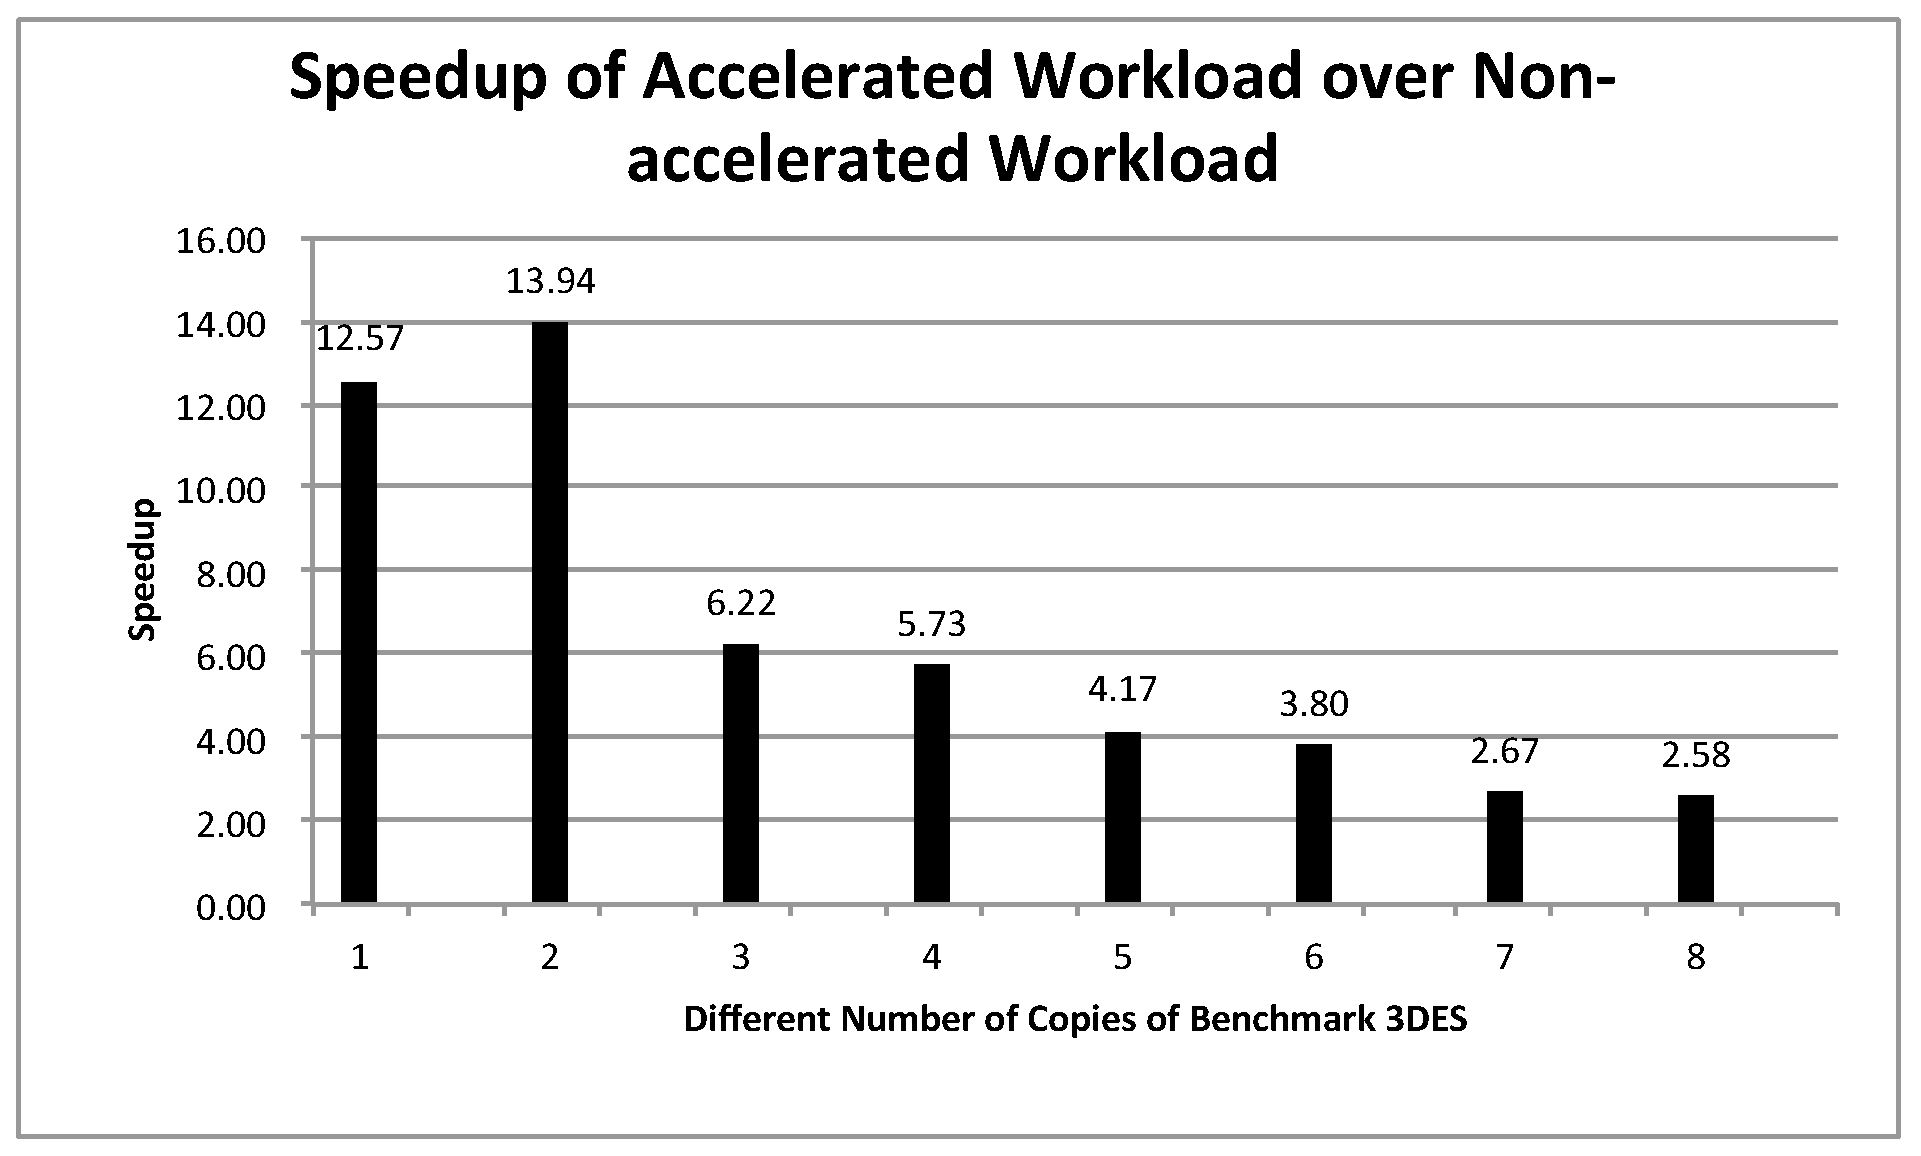
\includegraphics[width=4.5in]{Increase-Num-of-Apps}
    \caption{Speedup of Multiple Copies of a Single Workload Type}
    \label{fig_num_of_apps}
\end{figure}

\subsubsection{Speedup and Energy Efficiency of Workload Mixtures}

With a mixture of the workloads, the instantiation of accelerator
functions is subject to the run-time demands and the logic resource
constraints. We execute the synthetic workloads on {\em Transformer} with eight
cores and one reconfigurable logic unit of the size of an Xilinx
Spartan 3E. The workload's arrival follows either a Poisson process or
a back-to-back fashion.  We issue 100 thousand billion instructions of
the benchmark bundle and record the number of completed functions and
cycle times. 

\begin{figure}
    \centering
    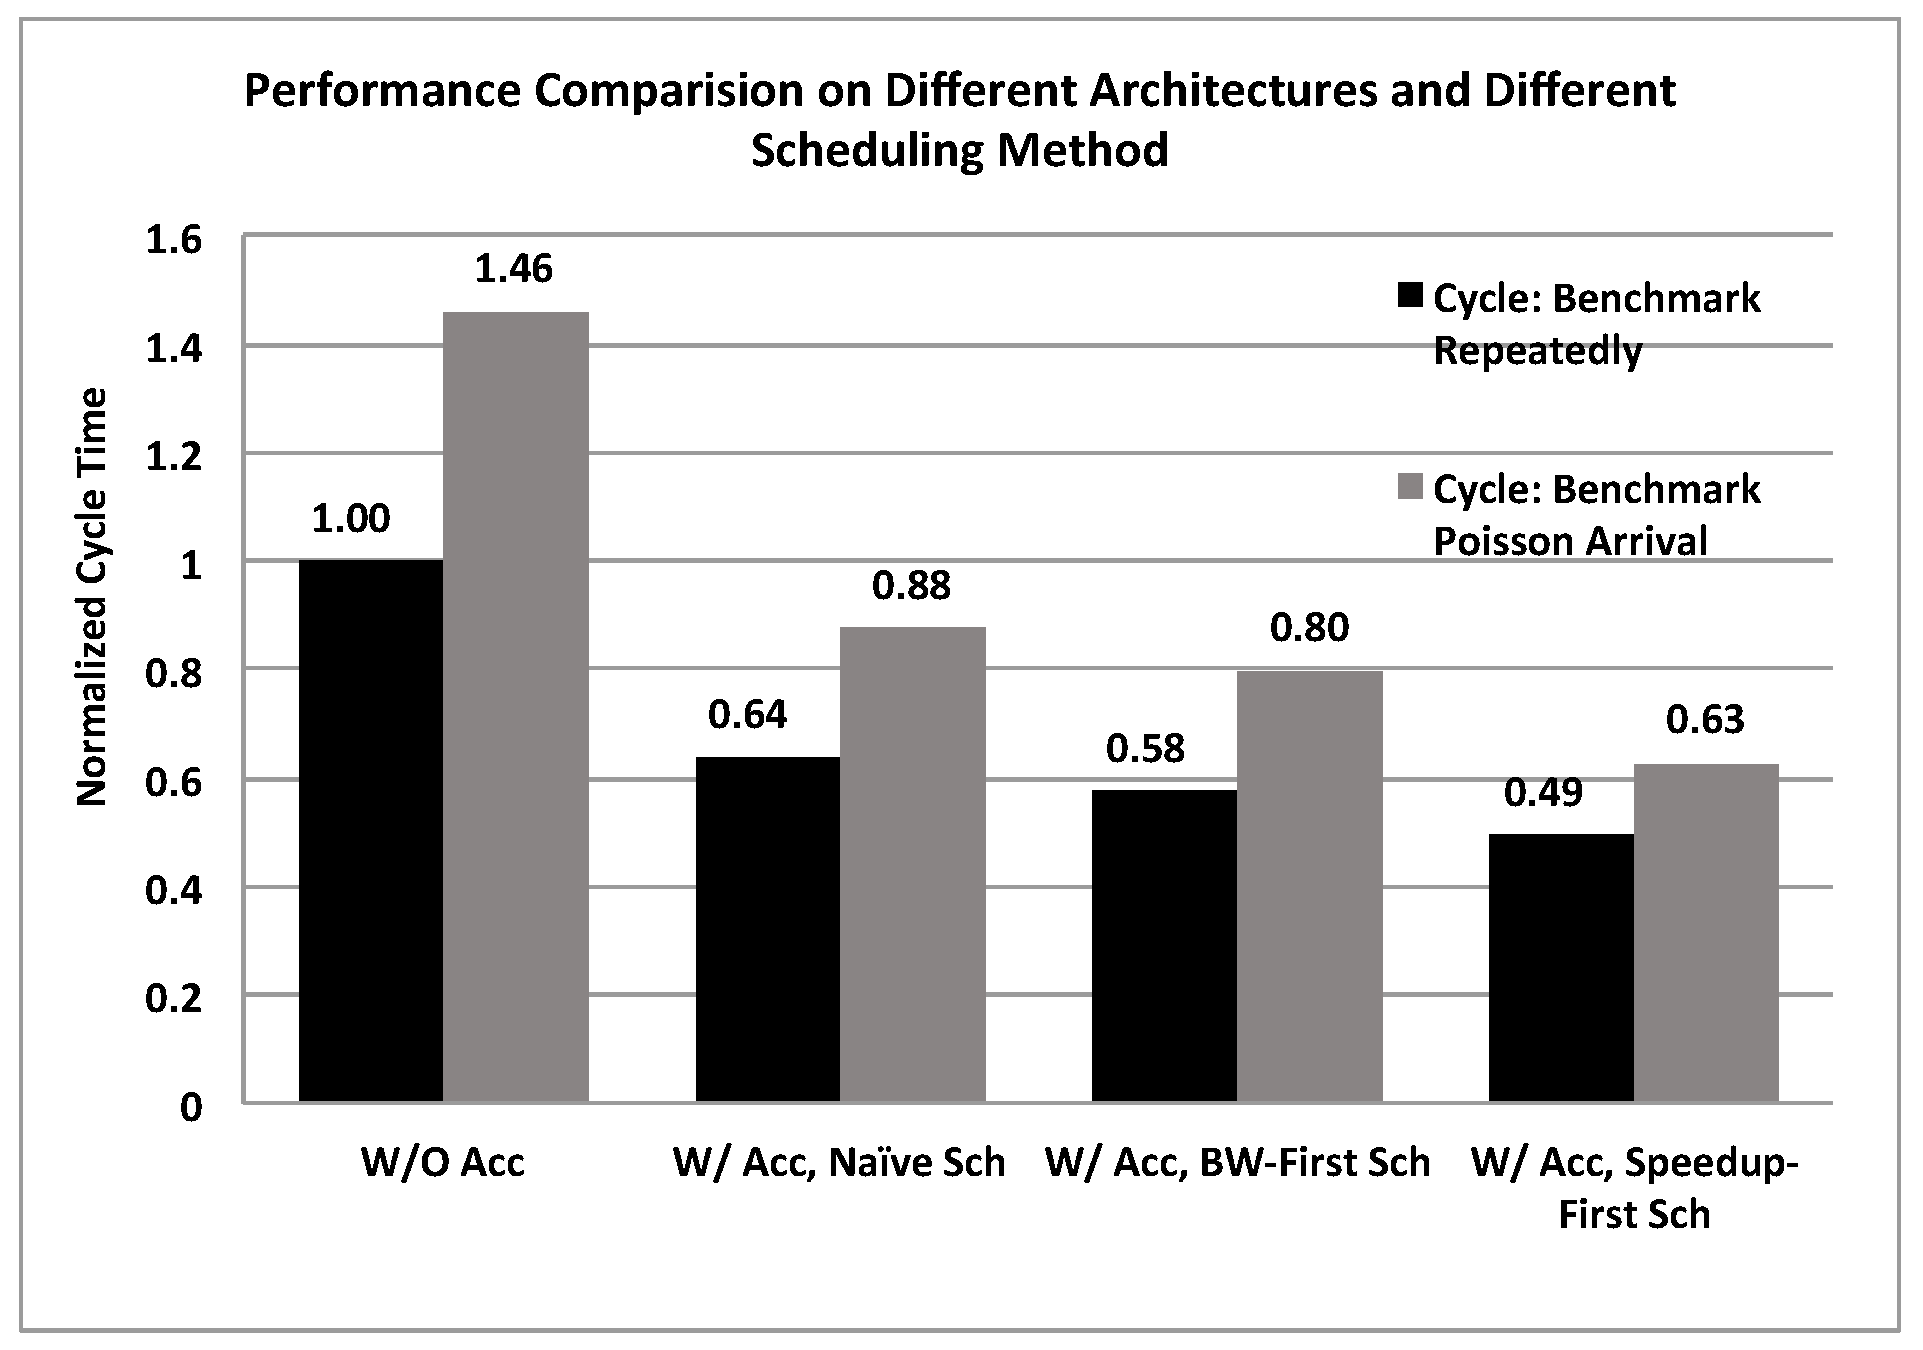
\includegraphics[width=4.5in]{Cycle-8core}
    \caption{Performance Comparison of Accelerated Architecture and Scheduling Algorithms.}
    \label{fig_8core_cycle}
\end{figure}

\begin{figure}
    \centering
    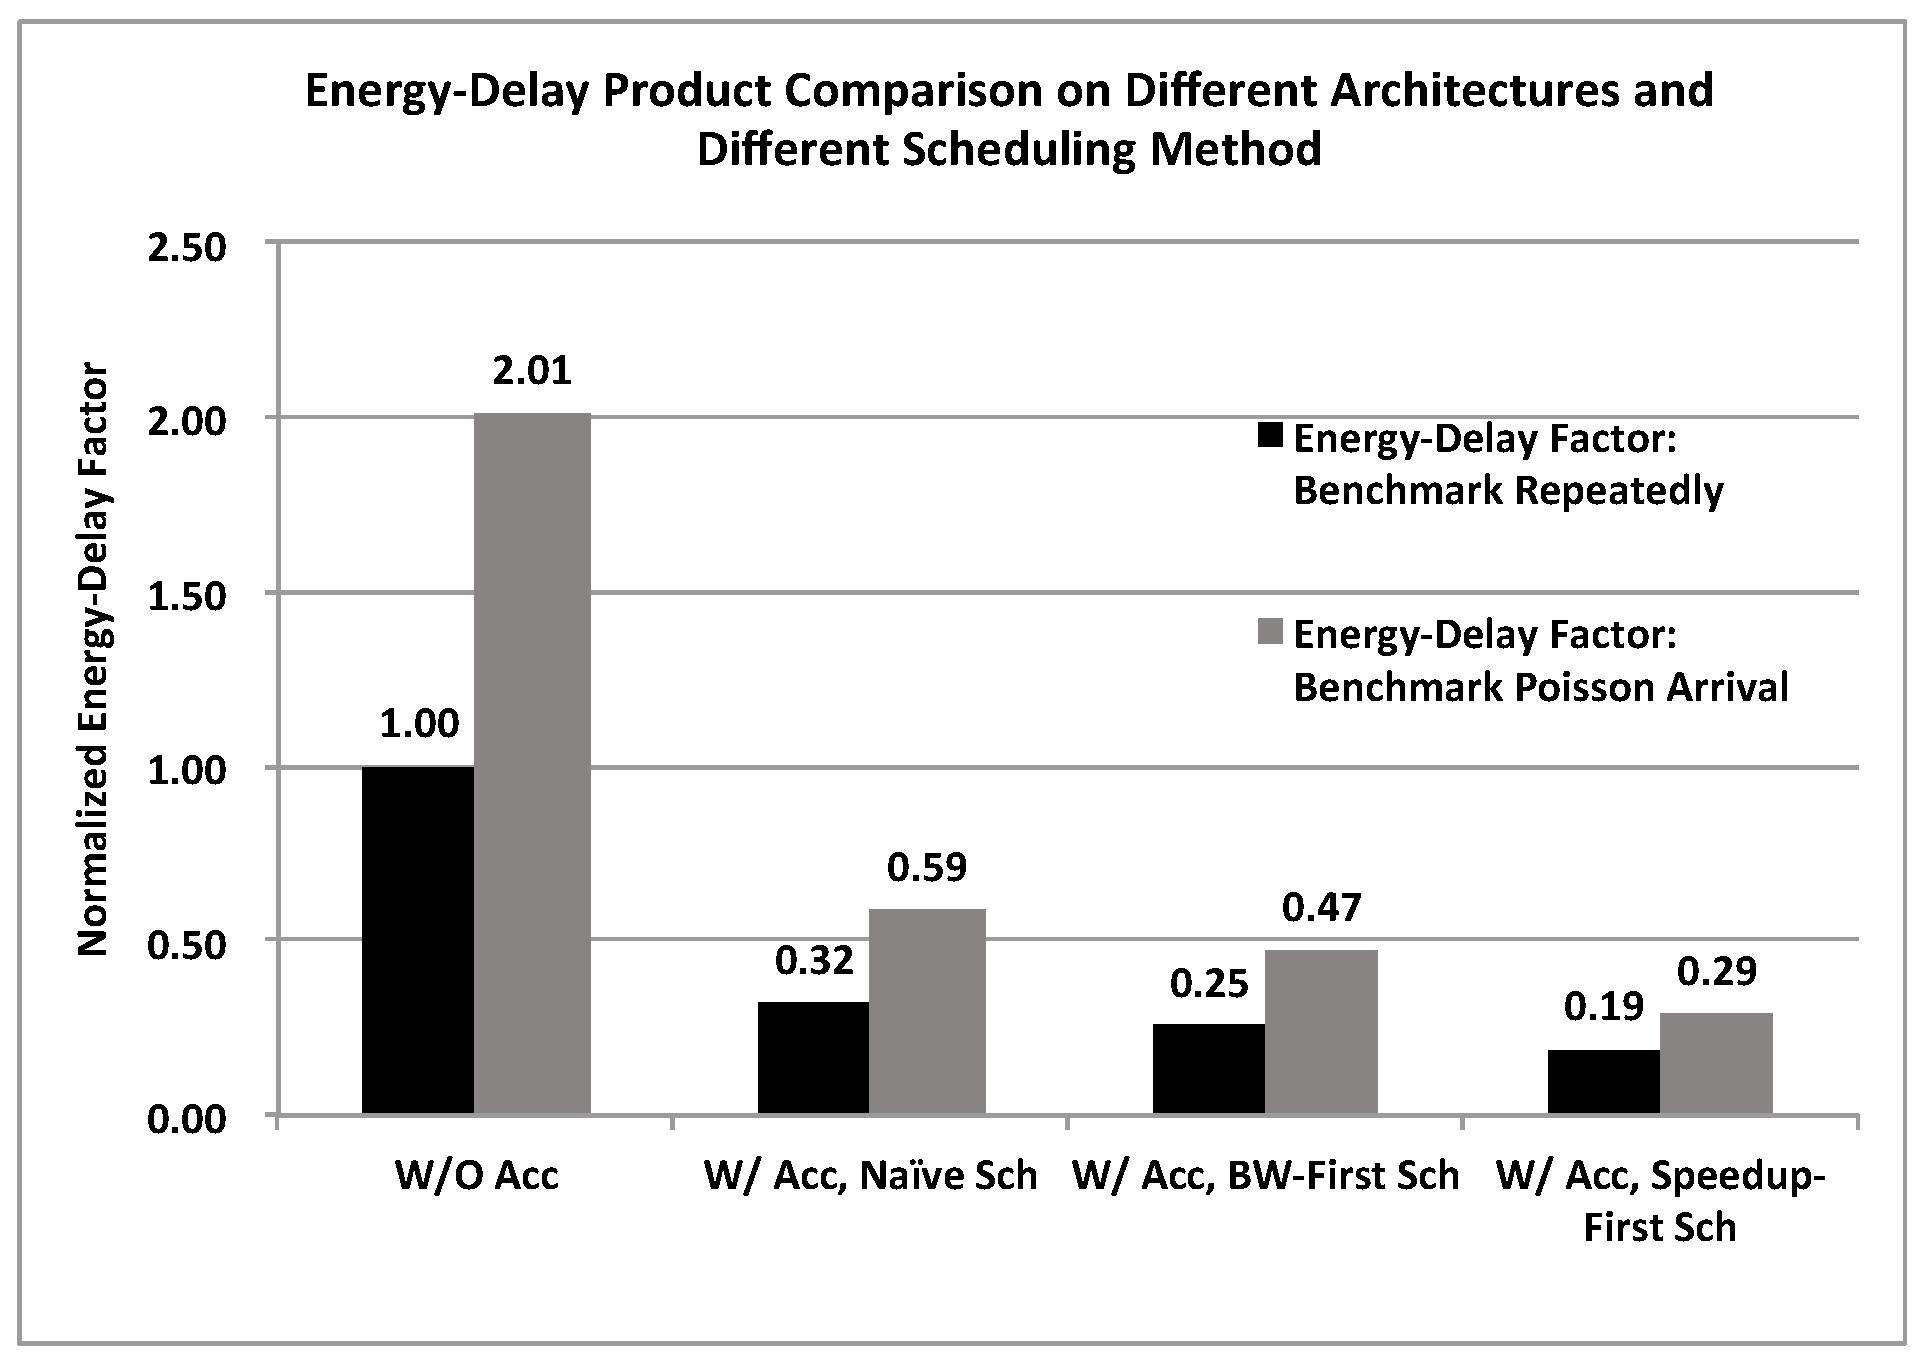
\includegraphics[width=4.5in]{Energy-Delay-8core}
    \caption{Energy-delay Product Comparison.}
    \label{fig_8core_energy_delay}
\end{figure}

In Figure \ref{fig_8core_cycle}, the x-axis denotes different architectures and scheduling methods, such as ``W/O Acc" (without accelerator), ``W/ Acc, 100\% Perfect" (with accelerator and 100\% perfect prediction accuracy of the incoming workloads), ``W/ Acc, Random" (with accelerator and randomly schedule incoming workload to either CPU or accelerators), ``W/ Acc, Acc-First" (with accelerator and schedule workload to accelerators with the first priority), ``W/ Acc, Naive" (with accelerator and profiling only),``W/ Acc, BW-First" (with accelerator and profiling plus Bandwidth First scheduling), and ``W/ Acc, Speedup-First" (with accelerator and Speedup First scheduling). The y-axis stands for the percentage of either performance gain or power efficiency gain.

If not considering the ideal Perfect Prediction scheduling, we can see the accelerated
architectures delivers up to 2.3x improvement on the performance
compared to a multicore architecture without an accelerator. It is
worth noting that such speedup is achieved on a highly dynamic
workload bundle of which the processor has no prior knowledge of the
workload types and arrival times. All the profiling is done at run-time and the
scheduling of the accelerator is autonomously performed by the
middleware (wrapper library). The workload following a Poisson arrival
process has longer execution time because there are idle cycles
between function calls. However, Poisson arrival provides more dynamic
combination of workload arriving at different time, and that's why we
observe a larger speedup (1.46/0.63$\simeq$2.3x) comparing with the
back-to-back arrival (1/0.49$\simeq$2x). 

The energy-delay product depicted in Figure
\ref{fig_8core_energy_delay} show that the power efficiency of {\em
 Transformer} improves by up to (2.01/0.29$\simeq$6.9x) as the workloads migrate to
energy-efficient accelerators due to the scheduling and run-time
reprogramming.

As compared with other different scheduling methods, we also find our profiling methods to be the optimal with the only exception of Perfect Prediction scheduling. For example, the Speedup-First scheduling method outperforms the Random scheduling and Acc-First scheduling with a speedup of 2.12 and 1.96 respectively and a energy-delay factor gain of 5.17 and 4.24 respectively. The results of Perfect Prediction scheduling are promising, however such ``perfect" prediction never happens with the huge dynamics of the workloads in real world. Though ``perfect" in prediction, the Perfect Prediction scheduling method does not yield ``perfect" utilization of the accelerator logics. As we argued in Section \ref{subsec_combo}, maximizing the utilization of reconfigurable logics is one of the contributions in our work to improve system performance and decrease the power consumption. The Bandwidth-First scheduling and the Speedup-First scheduling, on the contrary, take both accelerator size and performance gain into consideration. Thus, on one hand, Bandwidth-First and Speedup-First scheduling methods may not be able to compete with the 100\% Perfect Prediction in terms of the prediction accuracy, however on the other hand, their accelerator combination mechanism improves the whole system performance. As shown in Figure \ref{fig_8core_cycle}, Speedup-First scheduling resembles the performance of the 90\% Perfect Prediction scheduling and Bandwidth-First scheduling matches with the performance of 80\% Perfect Prediction scheduling. 

\subsubsection{Performance and Power Analysis with Various Time Window Sizes}
One of the basic parameter setups of the experiment is the choice of profiling time window $T$. As we mention in \ref{subsec_ranking}, bad choice of $T$ will bring either oversampling or inaccuracy. Thus, we implement a series of experiments to find the optimal range of $T$ that could be used for our benchmarks. 

We take the non-accelerated scenario as the baseline, and compare the performance and power efficiency gain of naive scheduling over the baseline with different profiling time window sizes. The experiment results are shown in Figure \ref{fig_time_window}.

Both performance and power efficiency gain increase when $T$ goes up from $1 ms$ to $100 ms$, stay in the plateau stage when $T$ locates around $100 ms$ to $1000 ms$, and sharply drop when $T$ goes beyond $1000 ms$, where the drop is caused by the accuracy loss of profiling method when down-sampling the benchmarks. According to the results, $[10 ms, 1000 ms]$ is a reasonable range to choose $T$ in our experiment. We also notice that the performance gain and power efficiency gain is still positive when $t = 1 ms$ tough sampling rate is the highest. That means the benefits of applying profiling outperforms the profiling overhead. 

\begin{figure}
    \centering
    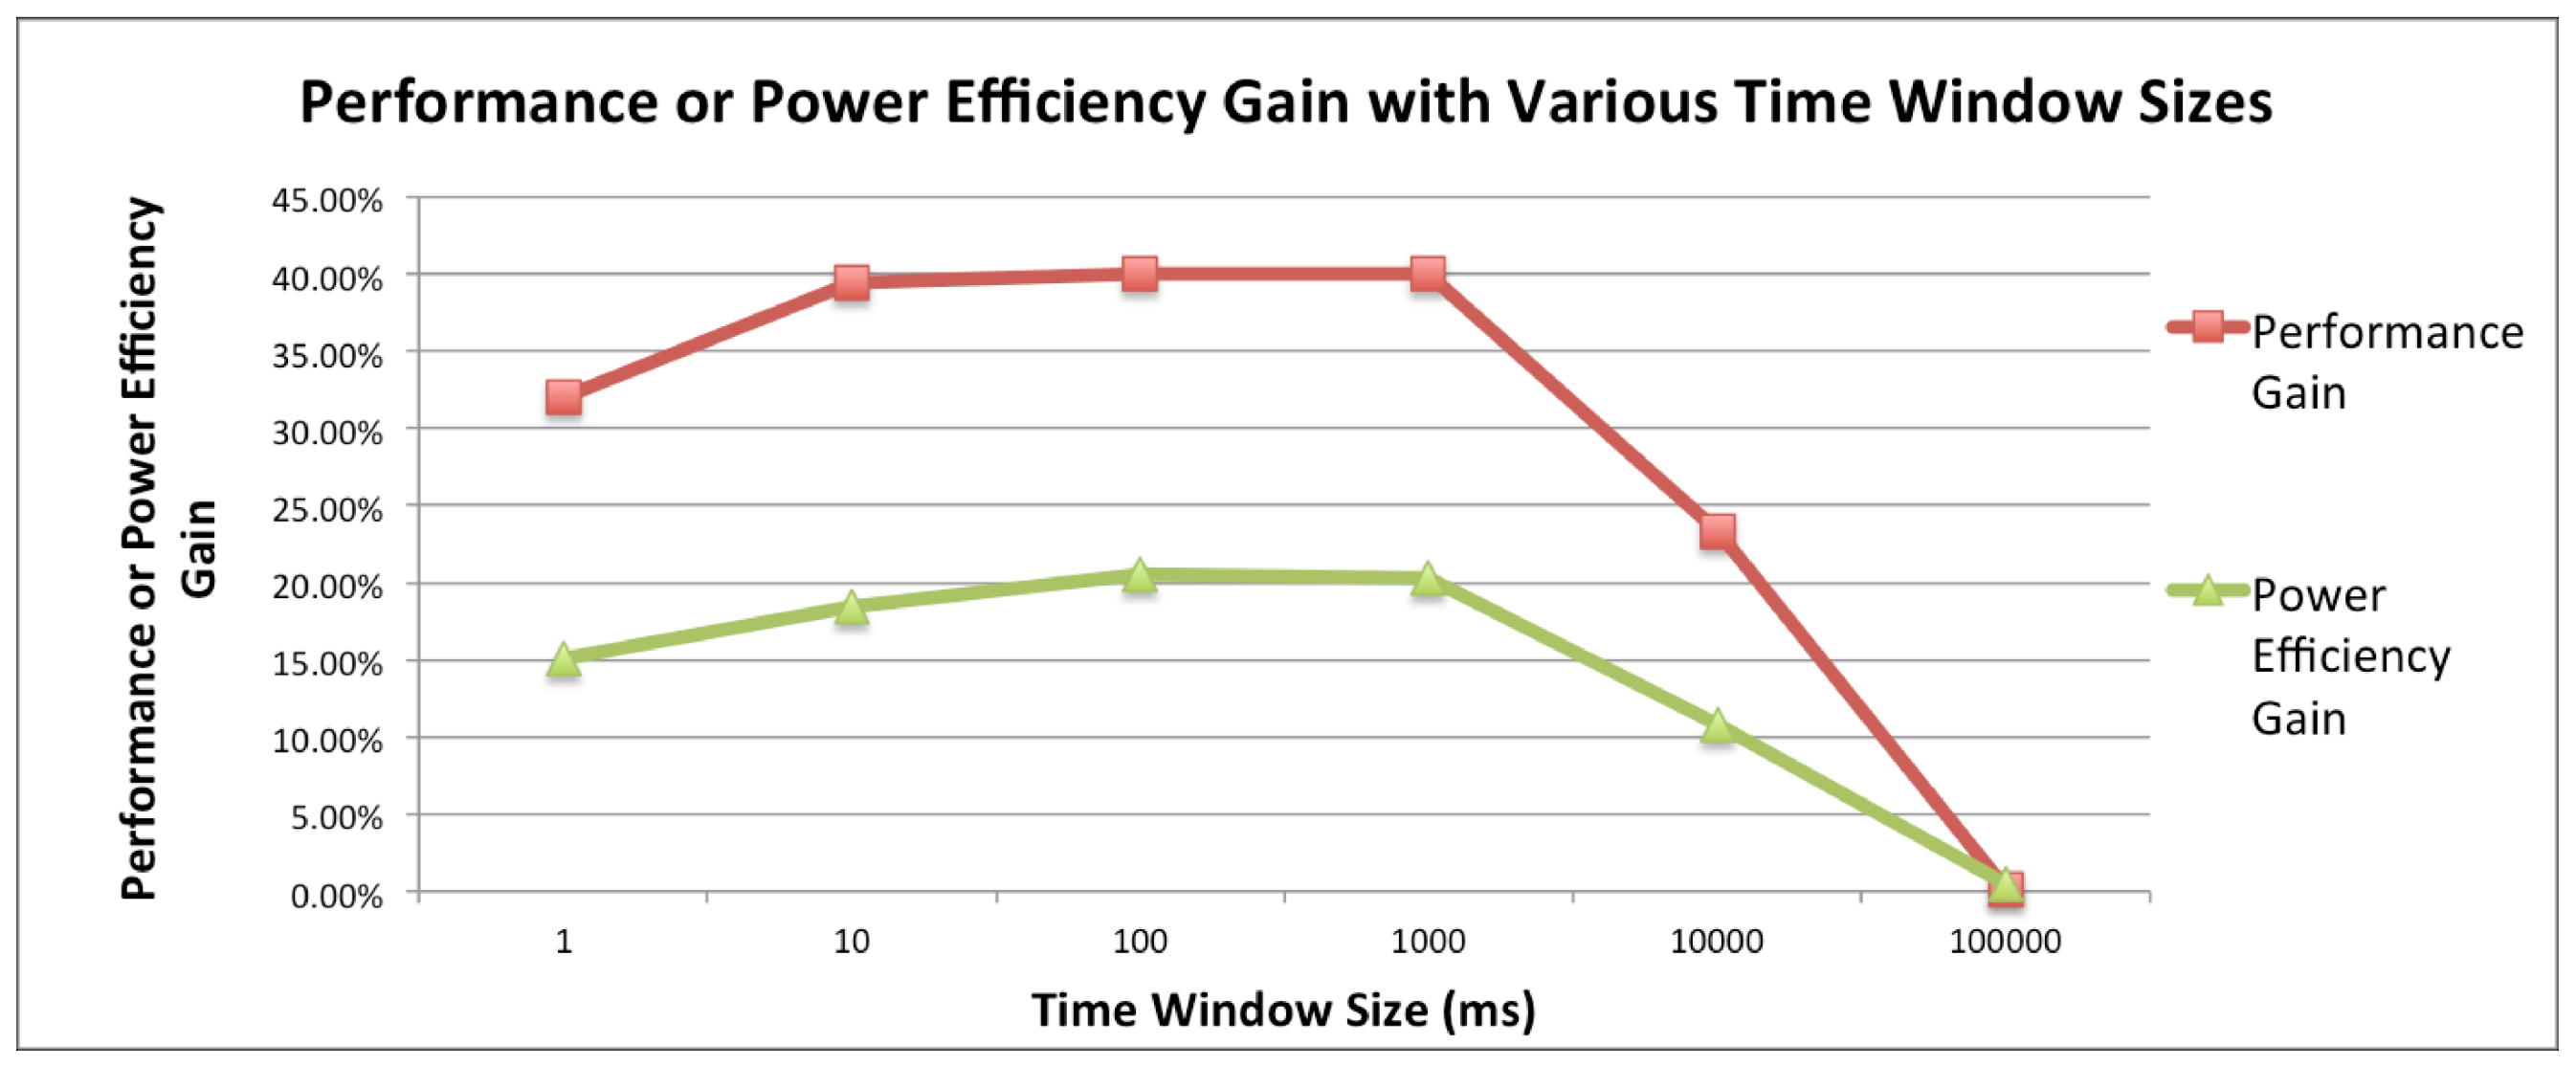
\includegraphics[width=4.5in]{Time-Window-Size}
    \caption{Performance and Power Analysis with Various Time Window Sizes.}
    \label{fig_time_window}
\end{figure}

\subsubsection{Impact of Accelerator Scheduling on Memory-bound vs
  CPU-bound Applications}

We study the impact of the two scheduling heuristics, bandwidth-first
and speedup-first, on different types of workloads, and compare the
heuristics with na\"{\i}ve scheduling (just use calculated priority
rank $P_x$).  We construct two workload bundles based on the memory
access intensity of benchmarks: memory-bound (bandwidth over 500MB/s
in Table \ref{tbl_benchmark}) and CPU-bound.

By design,
bandwidth-first strategy prioritizes the utilization of memory
bandwidth, which inherently gives memory-bandwidth hungry benchmarks
more chances to take advantage of the accelerator logics. As a result,
this strategy outperforms speedup-first for memory-bound
applications as shown in Figure \ref{fig_mem_bound}. On the other hand,
CPU-bound applications benefit more from speedup-first
scheduling strategy as depicted in Figure \ref{fig_cpu_bound}.

\begin{figure}
    \centering
    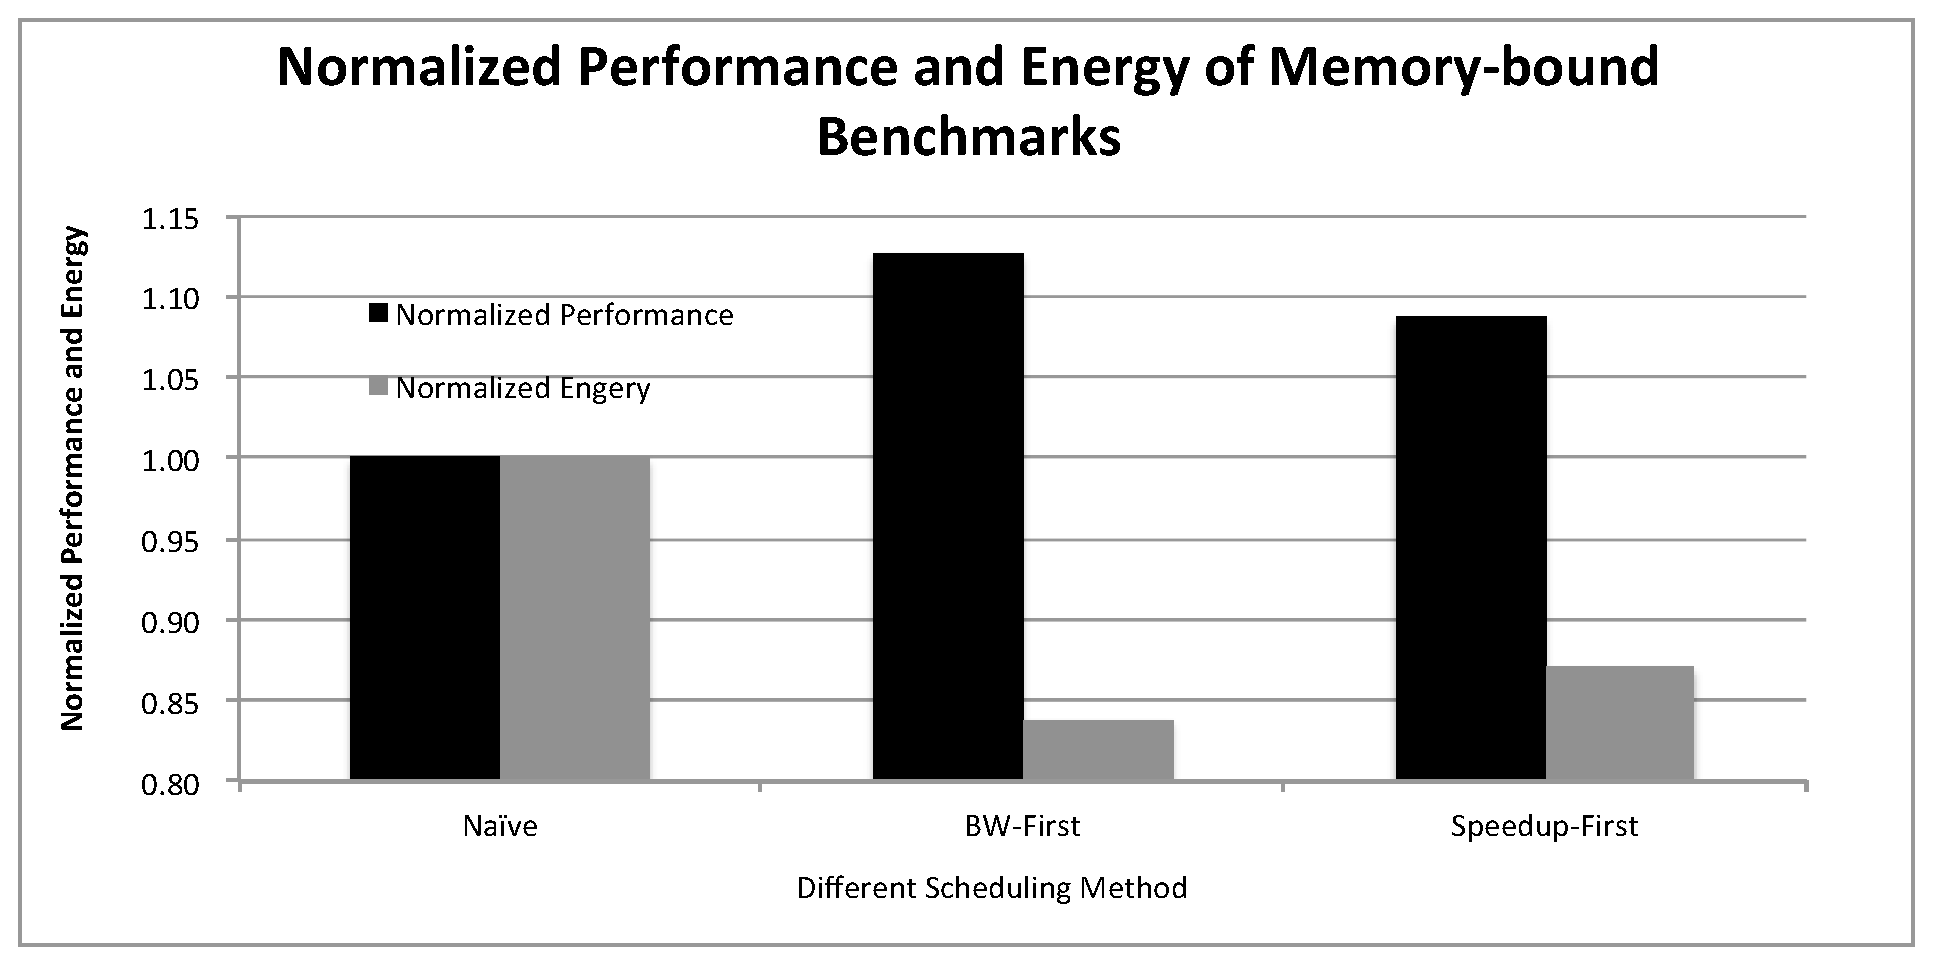
\includegraphics[width=4.5in]{Memory-Bounded}
    \caption{Performance and Energy Consumption of Memory-bound Benchmark Group.}
    \label{fig_mem_bound}
\end{figure}

\begin{figure}
    \centering
    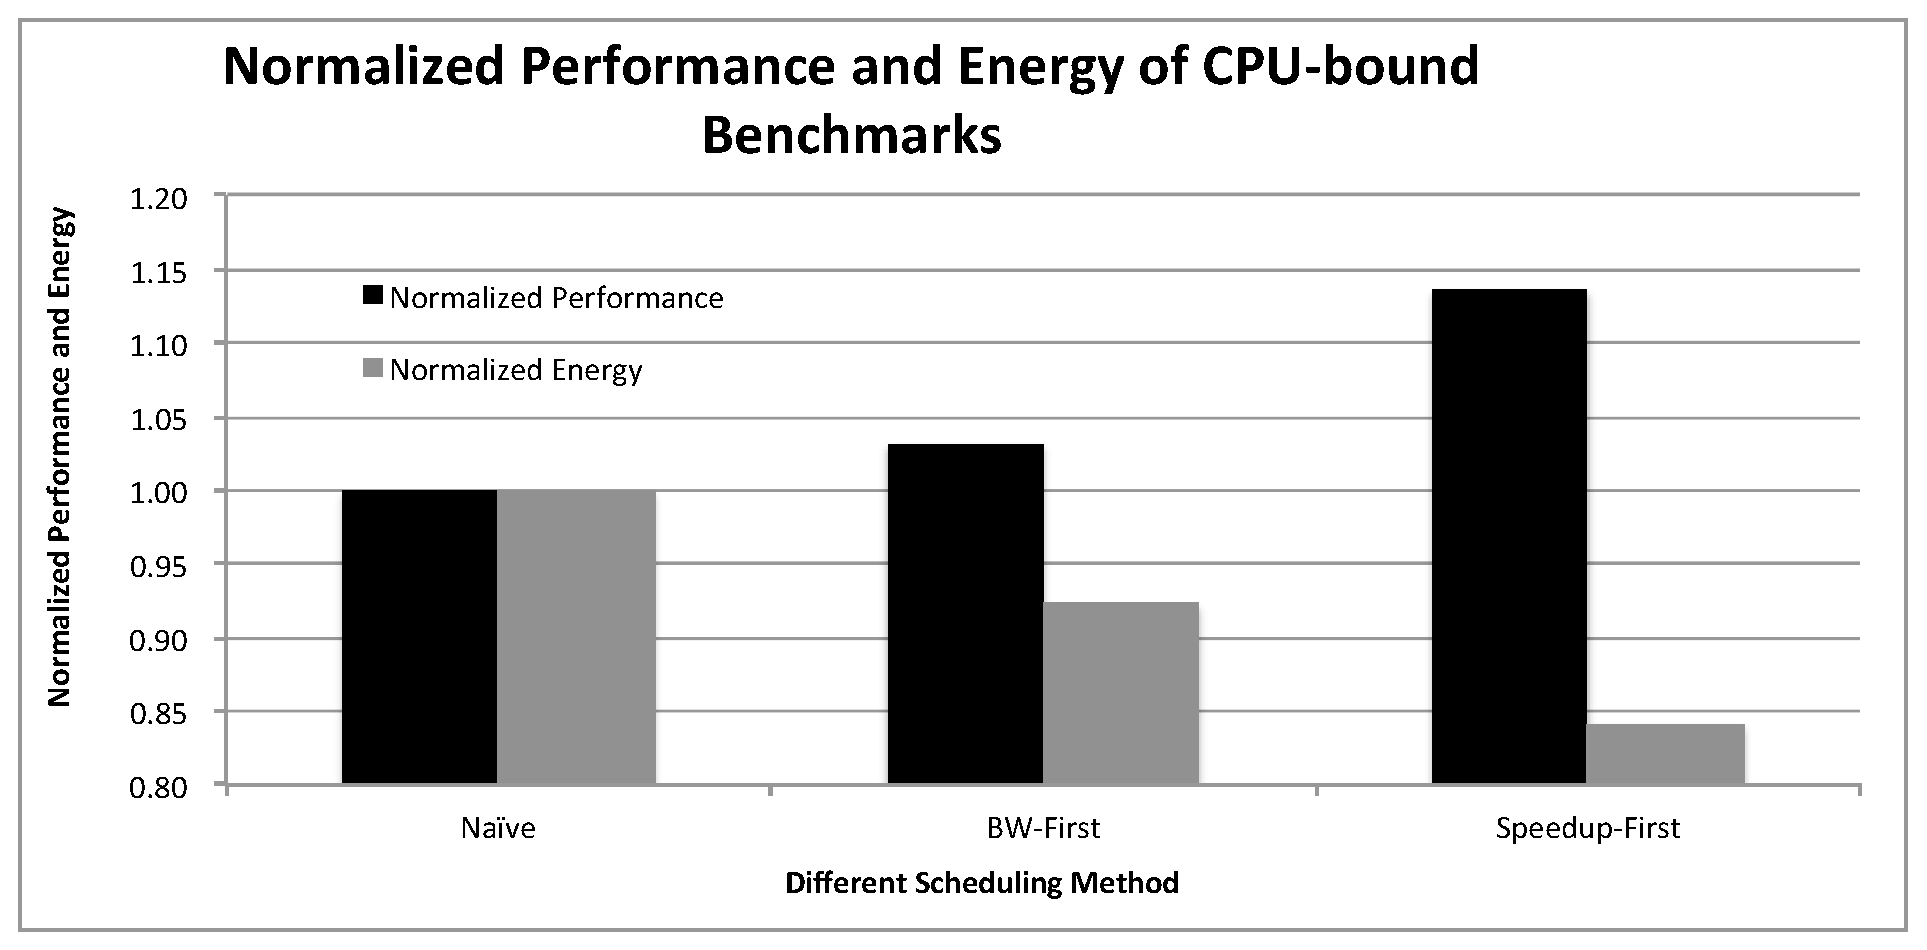
\includegraphics[width=4.5in]{CPU-Bounded}
    \caption{Performance and Energy Consumption on CPU-bound Benchmark Group.}
    \label{fig_cpu_bound}
\end{figure}


\subsubsection{Chip Area Allocation}

It is very interesting to understand how we should allocate chip
area to cores and programmable accelerators, given a limit on the chip
area. We vary the number of cores and the size of the
reconfigurable logic to explore the design space. Figure
\ref{fig_core_acc_ratio} is obtained by changing the core and
accelerator area ratio given a total area equivalent to four cores
plus a Spartan 3E like reconfigurable logic unit (default
accelerator size). As the area of an Atom core is about
    a quarter of Spartan 3E, the combinations of cores and reconfigurable
logics are 8:0, 6:0.5, and so on. It is very interesting to see
 5:0.75 gives the optimal performance gains while more accelerator
logics keep improve the energy efficiency. While such ratio is
specific to the workloads and should be cautiously generalized, 
our results show that it is important to
investigate the design space to explore the best possible
combinations of cores and accelerators. 

\begin{figure}
    \centering
    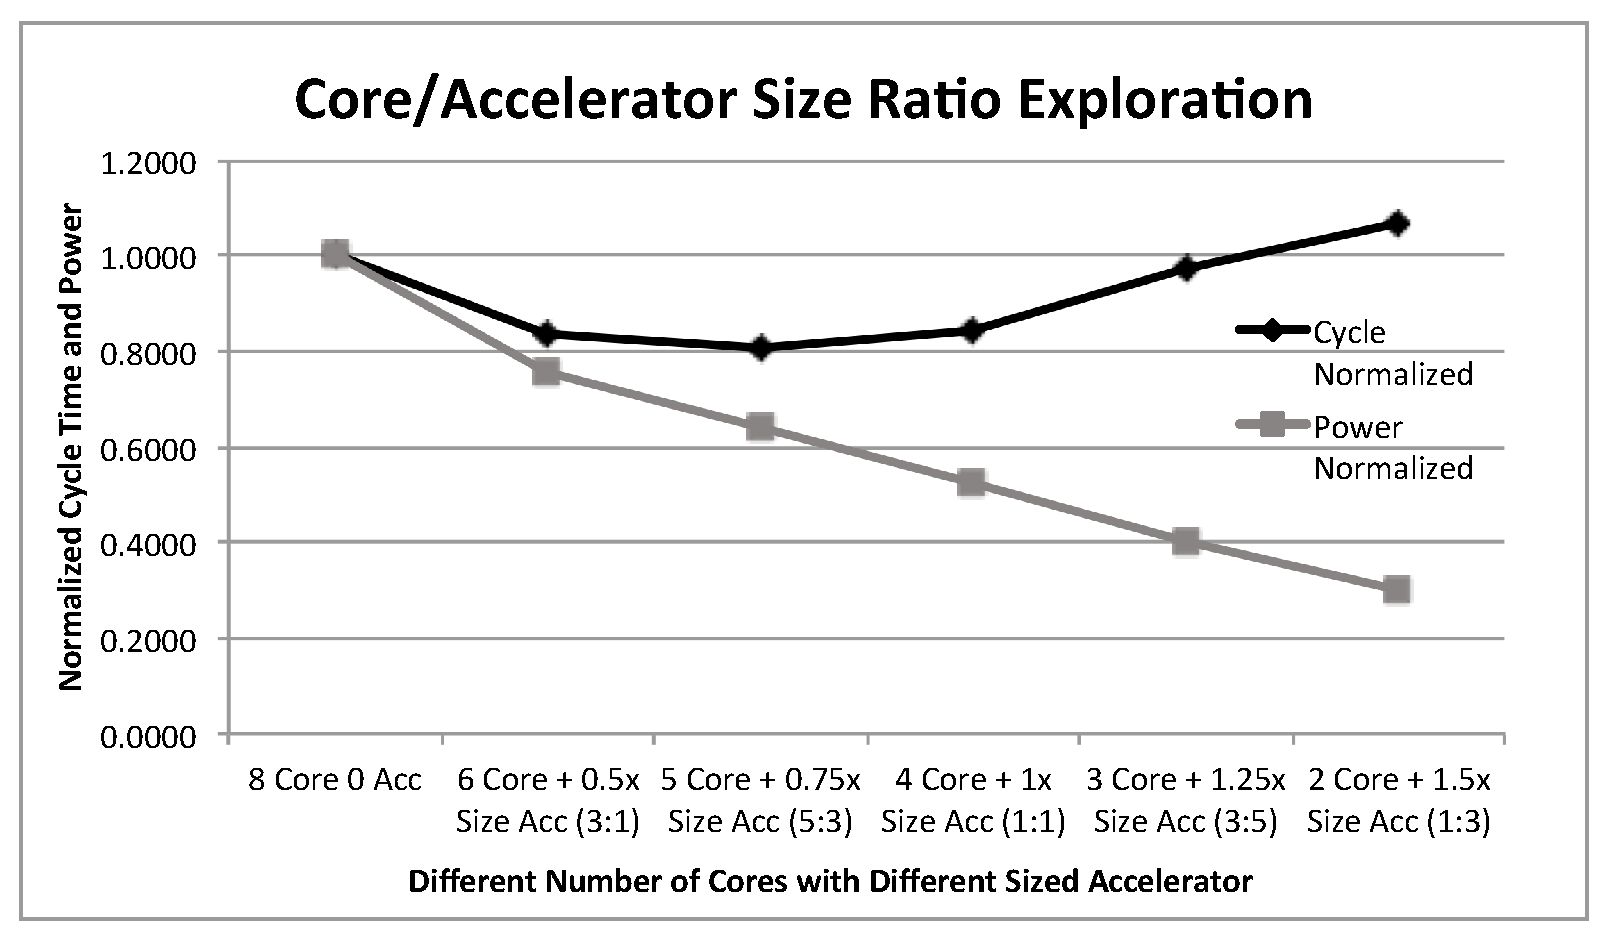
\includegraphics[width=4.5in]{Core-Acc-Size-Ratio}
    \caption{Performance and Power with Different Core/Accelerator Ratios.}
    \label{fig_core_acc_ratio}
\end{figure}

\subsubsection{System Parameter Analysis}


\subsubsection{Utilization of Reconfigurable Resources}

Figure \ref{fig_acc_timeline} shows a sample of the run-time
reconfiguration process on the {\em Transformer}. The x axis is the
scheduling time window, and the y axis is the number of acceleration
functions instantiated on the SoC. Figure \ref{fig_acc_timeline}
reveals the dynamics of the workload and how {Transformer} adapts its
resources to demanding functions. Figure \ref{fig_logic_timeline}
illustrates how the utilization of various resources within the
reconfigurable logic changes over time.

Figure  \ref{fig_acc_timeline}  also validates the advantages of run-time
configuration over fixed accelerators. We observe the maximum number of each
accelerators as: 3DES, SURF, Segmentation and Smithwaterman - 1
instantiation, IDSI and SLAM-J - 2 instantiations, SLAM-C and Jacobi -
3 instantiations. To achieve the same performance, the total logics we
would need if we rely on fixed onchip accelerators are: SLICE - 17848, FF
- 14511, LUT - 13192, BRAM - 255. That is, we would need at least 3.8 times
more SLICE and 12.75 times more BRAM to perform comparably as {\em Transformer}. 
This is a example for your.


\begin{figure}[ht]
    \centering
    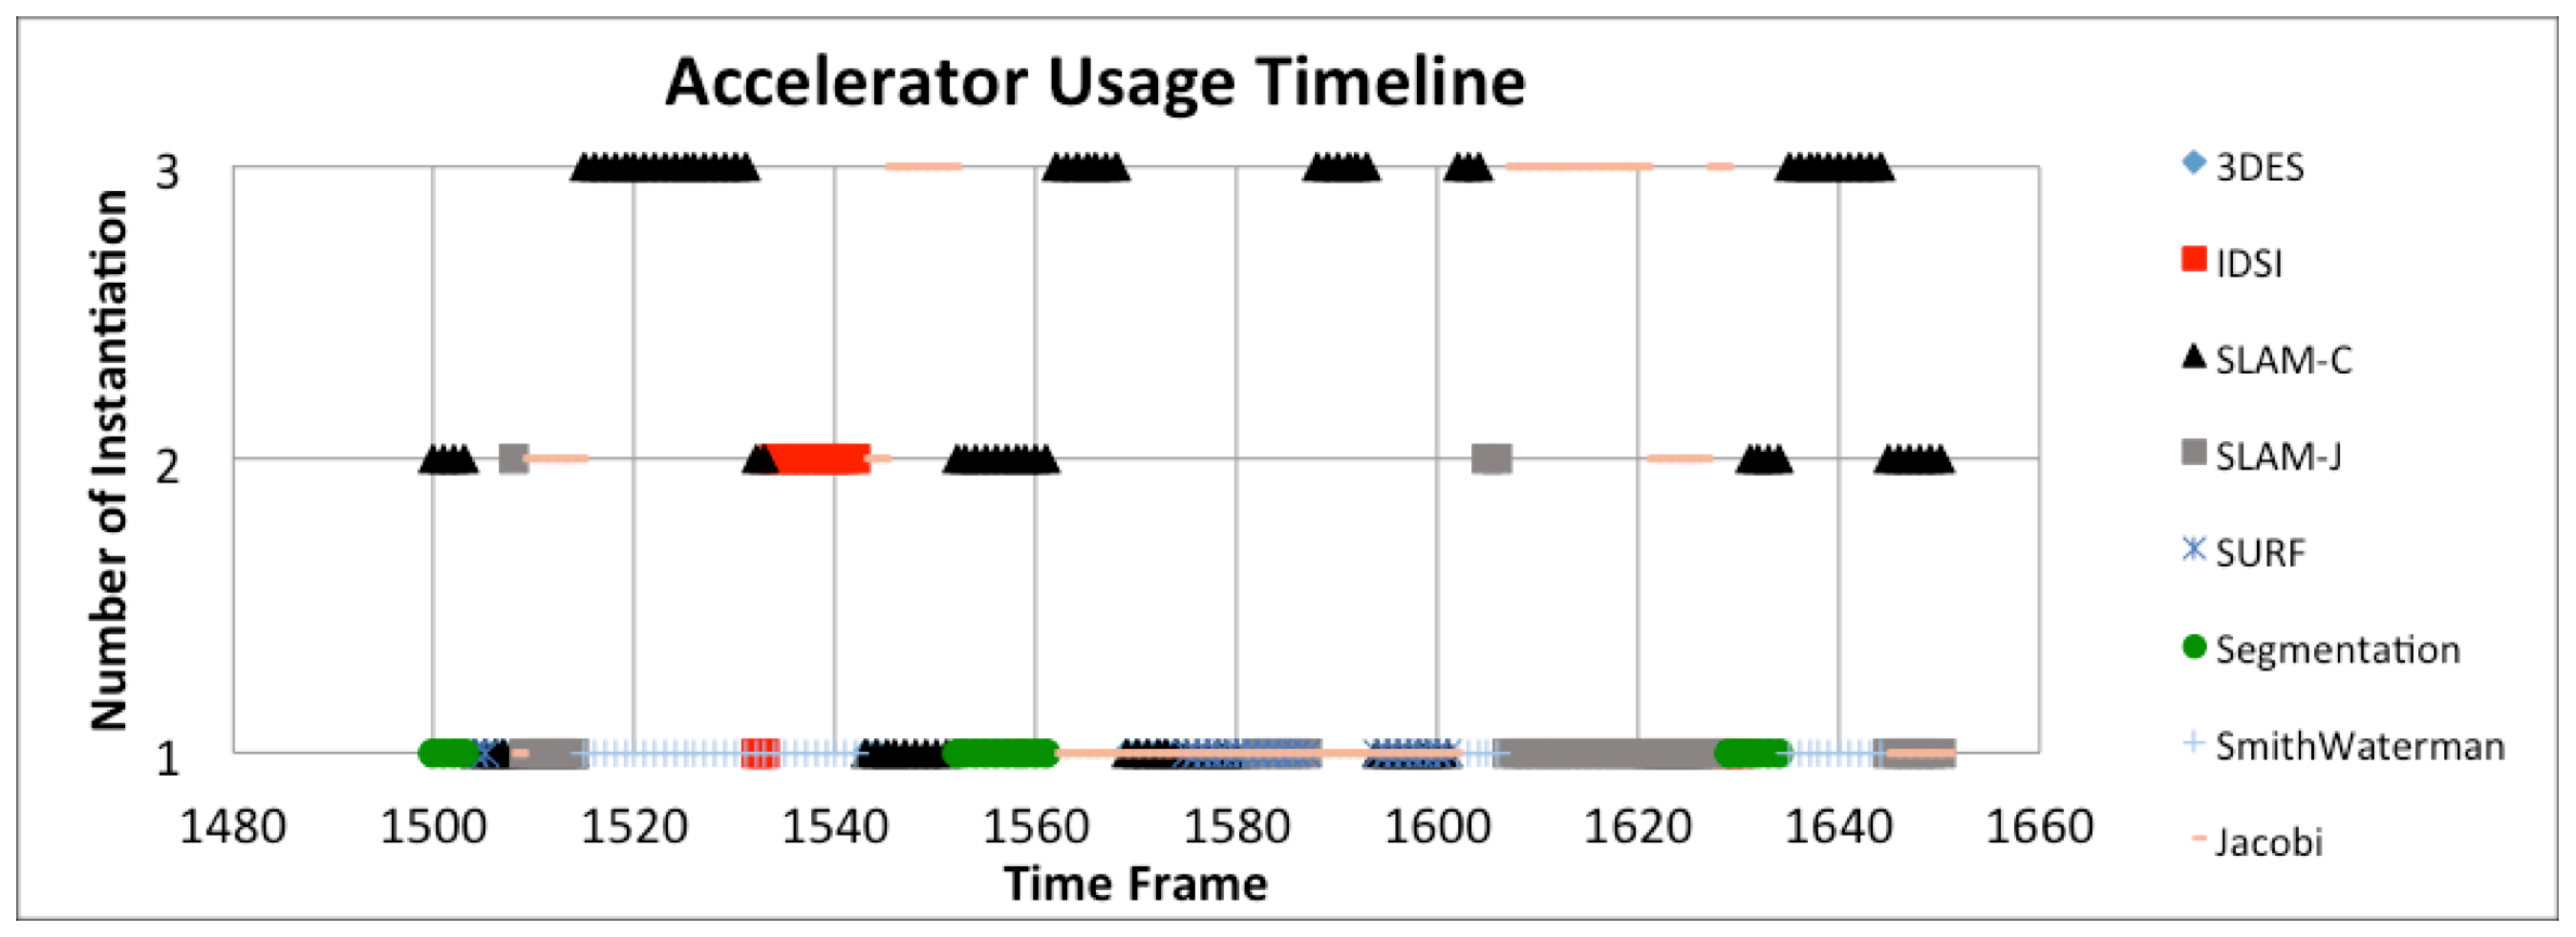
\includegraphics[width=6.0in]{Acc_timeline}
    \caption{Accelerator Usage Timeline.}
    \label{fig_acc_timeline}
\end{figure}

\begin{figure}[ht]
    \centering
    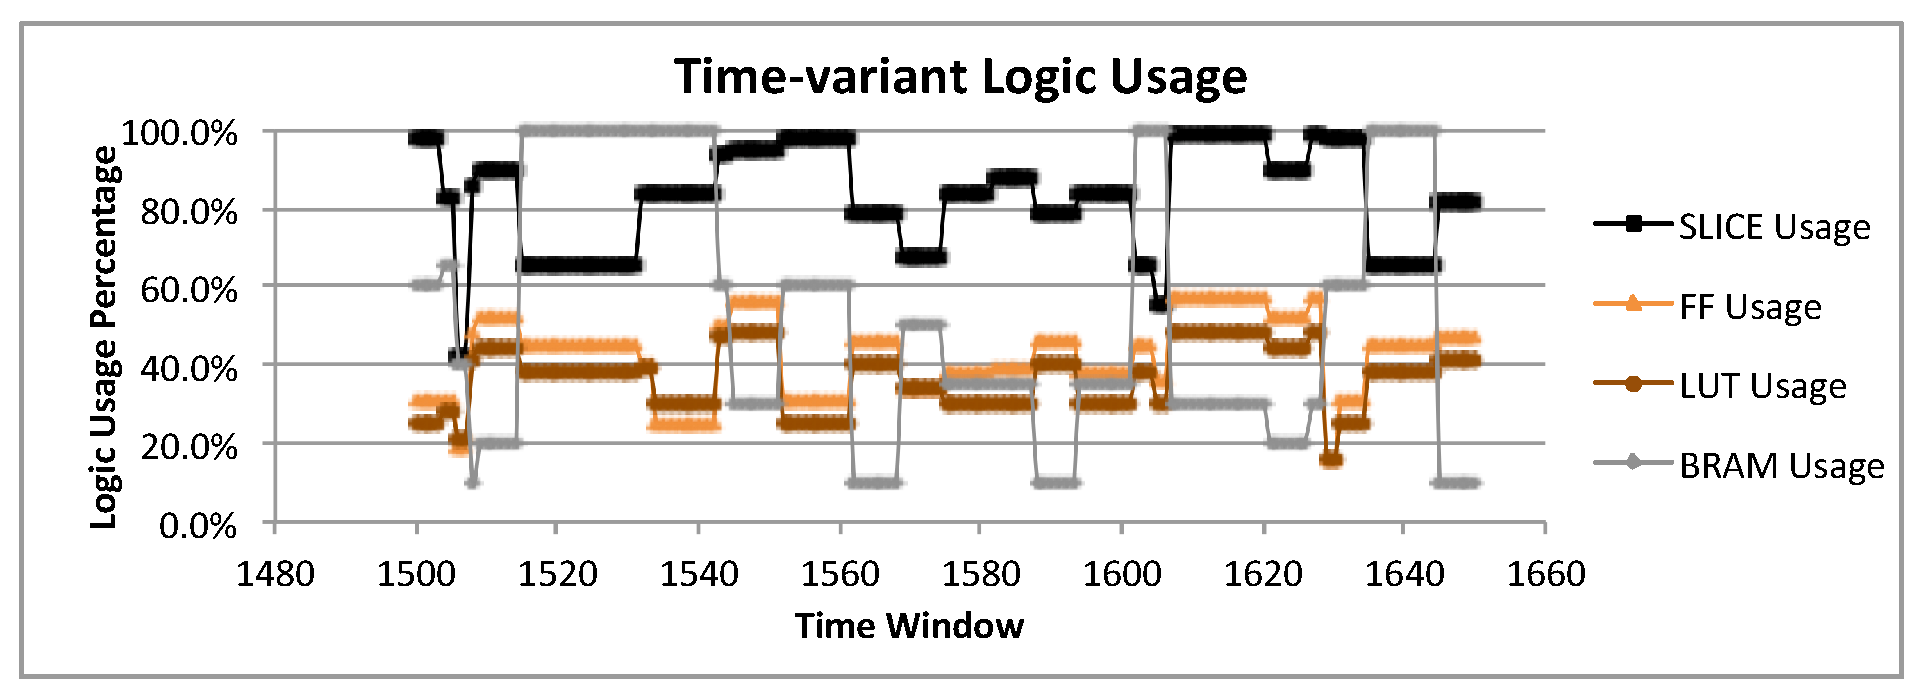
\includegraphics[width=6.0in]{Logic-Usage-Timeline}
    \caption{Total Logic Usage Timeline.}
    \label{fig_logic_timeline}
\end{figure}
